\setcounter{chapter}{9}
\setcounter{section}{0}
\setcounter{figure}{0}
\setcounter{equation}{0}
\setcounter{table}{0}
\chapter*{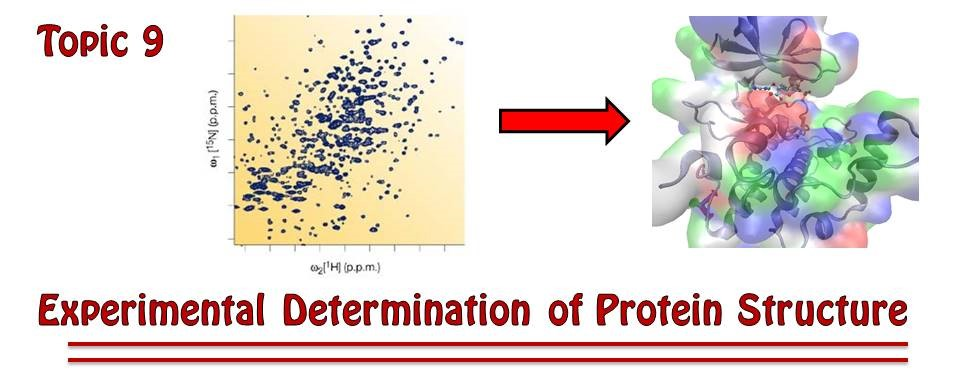
\includegraphics[width=\textwidth]{./figures/Topic9/Topic9.jpg}}
\addcontentsline{toc}{chapter}{Topic 9: Experimental Determination of Protein Structure}

\section{Introduction}

Funded by the U.S. Department of Energy and the National Institute of Health, the monumental Human Genome Project was completed in 2003, providing a complete sequence of the 3 billion chemical base pairs and the 25,000-odd genes that make up our genetic map, or genome.  Like a blueprint for a house, the genome tells us how to create a human being -- if we can learn to read it.  The next hurdle for scientists is interpretation.

Each gene codes for a specific protein, and each protein performs a specific function in the cell.  Some proteins provide the structure of skin, bones, and hair; other proteins transport molecules across membranes; and still other proteins facilitate important chemical reactions.  Now that the human genome is complete, we want to know which gene codes for which protein and what that protein does in the body.  Given the tight relationship between structure and function in biology, it becomes necessary to determine the three-dimensional shape of a protein before we can ascertain what the protein does in the cell.  

As of January 2017, scientists around the globe had catalogued the structures of about 116,000 proteins and other biological macromolecules.  These structures, known to atomic resolution, are deposited in and accessed from the RCSB Protein Data Bank (\href{http://www.rcsb.org/pdb/statistics/holdings.do}{http://www.rcsb.org/pdb/statistics/holdings.do}).  Figure \ref{Fig9-1} shows that the number of known structures has exploded in recent years as more powerful experimental techniques have been developed.
\begin{figure}[h]
	\centering
	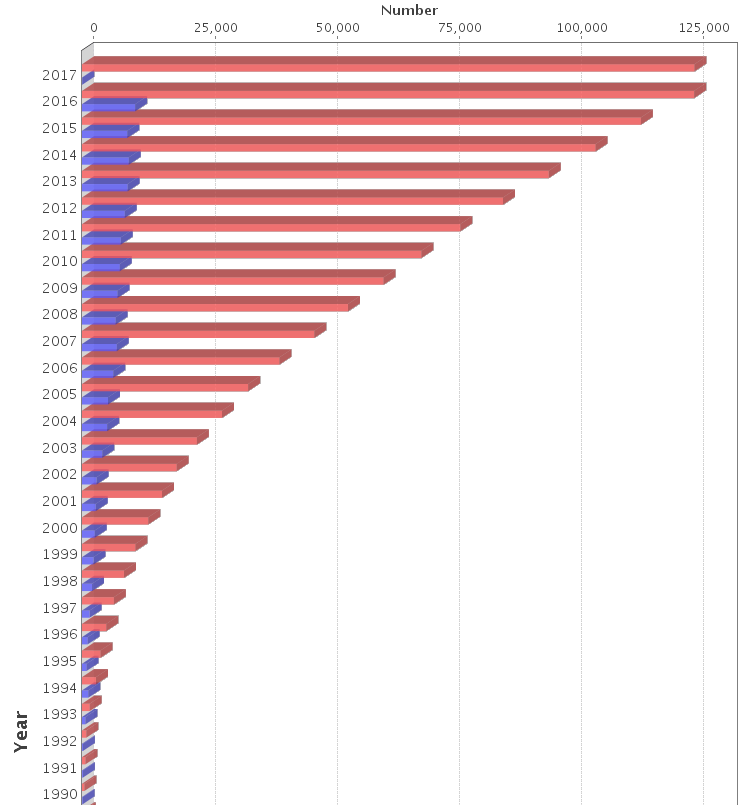
\includegraphics[width=3.5in]{./figures/Topic9/Fig9-1.png}
	\caption{As protein structures have become easier to solve in recent years, the total number of known structures (marked in red) has increased tremendously. The marks in blue represent yearly increases in structures reported.}
 	\label{Fig9-1}
\end{figure}

There are two principal techniques used to determine protein structure: X-ray Crystallography and Nuclear Magnetic Resonance (NMR) Spectroscopy.  Historically, x-ray crystallography has been the tool of choice for structural studies -- nearly 90\% of all structures have been solved with it.  But, NMR spectroscopy has gained immense popularity in the last decade and is now mainstream as well.  Because they provide complementary information, these methods are extremely powerful when used together.  
As we shall see, x-ray crystallography supplies information about the location of heavy atoms like carbons, oxygens, nitrogens, and heavy metal ions, while NMR gives the relative distance between pairs of hydrogen atoms or between a hydrogen atom and a carbon or nitrogen atom.  X-ray crystallography allows the structures of large proteins or complexes of proteins to be solved with great accuracy, but it is not useful for studying their dynamic properties since the technique requires the protein to be crystallized.  Crystal growth is extremely difficult and requires both luck and skill.  NMR, on the other hand, allows us to study proteins in solution, helping us to understand how they act {\it in vivo}.  However, most proteins over about 40 kDa have proved difficult to characterize by this method (1 Dalton = 1 amu/mol = $1.6605\times10^{-24}$ g/mol; 40 kDa = 40,000 amu/mol).
The following sections will give the basic principles behind x-ray crystallography and NMR spectroscopy, as well as a flavor for how the data acquired by each method is analyzed.  

\section{X-Ray Crystallography}

X-ray crystallography relies on the scattering of x-rays from electrons.  With wavelengths on the order of $\text {\AA ngstr{\"o}ms}$ (10$^{-10}$ m), an x-ray beam interacts strongly with the electron clouds of individual atoms in a crystallized protein, producing diffraction patterns that can be observed on a photographic plate. 

In any crystallography experiment, the first step is to prepare the sample.  This involves expressing and purifying the protein, concentrating it (2--50 mg/mL), and growing crystals.  Since proteins are large and irregular in shape, they do not fit well into a tight crystal structure; for this reason, the crystals are fragile and sensitive to changes in their environment.  Good crystals are a few tenths of a millimeter across in all dimensions. In Fig.~\ref{Fig9-2}, the crystals have been magnified approximately 100x.
\begin{figure}[h]
	\centering
	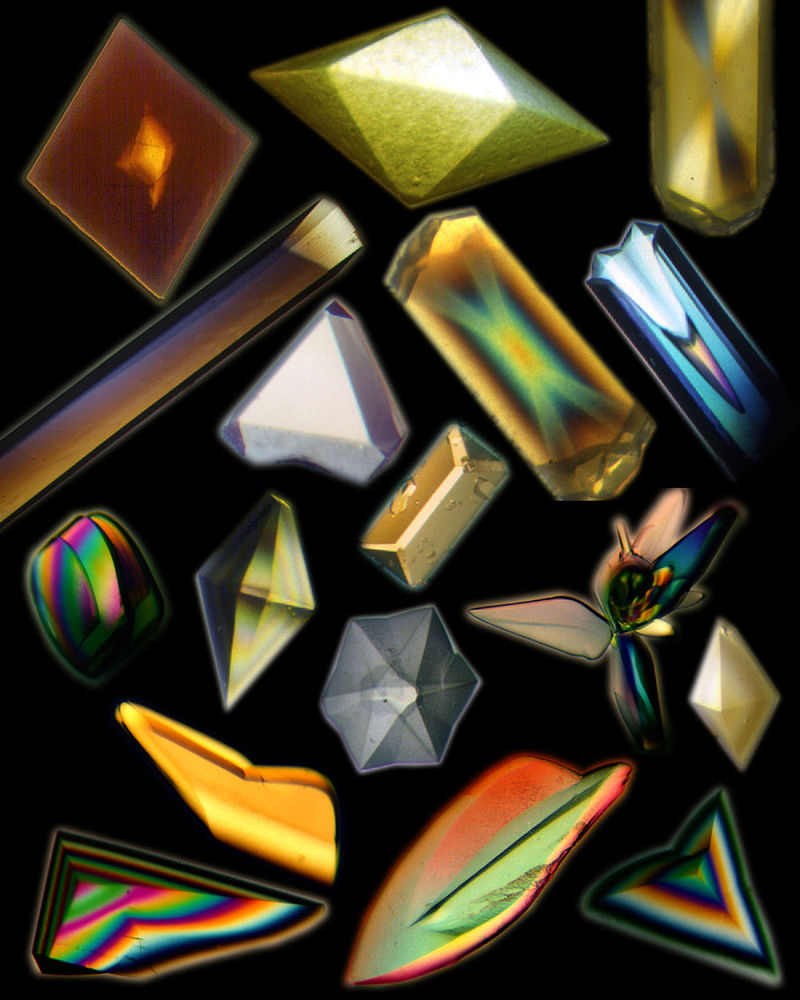
\includegraphics[width=3.0in]{./figures/Topic9/Fig9-2a.jpg}
	\caption{Examples of protein crystals grown in space. \href{https://en.wikipedia.org/wiki/Protein\_crystallizationl}{https://en.wikipedia.org/wiki/Protein\_crystallization}}
 	\label{Fig9-2}
\end{figure}
After quality crystals are obtained, they are placed in front of a powerful x-ray beam with a well-defined wavelength.  This requires a trip to a synchrotron -- a machine that accelerates a charged particle (often an electron) to nearly light speed and uses large magnets to guide it around an enormous circular tunnel.  As the electron spins around the circle, it ejects the intense x-ray beams needed by crystallographers.  To avoid crystal degradation from exposure to the intense radiation, the sample is often cooled to cryogenic temperatures ($\sim$125 K) before being exposed to the beam.
\begin{figure}[h]
	\centering
	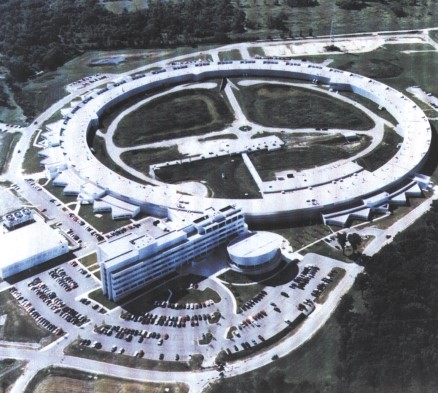
\includegraphics[width=2.5in]{./figures/Topic9/Fig9-3.jpg}
	\caption{An aerial view of the Advanced Photon Source at Argonne National Laboratory near Chicago. \href{http://www.nigms.nih.gov/news/science\_ed/structlife/chapter2.html}{http://www.nigms.nih.gov/news/science\_ed/structlife/chapter2.html}}
 	\label{Fig9-3}
\end{figure}
As x-rays scatter from the electrons of the protein, photographic or other imaging plates record the complex diffraction patterns. Figure \ref{Fig9-4} is one of many such scattering patterns for myoglobin, the first protein to be structurally characterized back in 1959.
\begin{figure}[h]
	\centering
	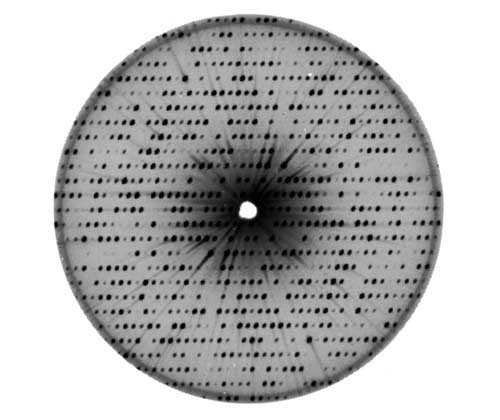
\includegraphics[width=3.5in]{./figures/Topic9/Fig9-4.jpg}
	\caption{A scattering pattern from myoglobin.}
 	\label{Fig9-4}
\end{figure}
The position of each spot on the plate depends on the arrangement of atoms in the sample.  Consider the simple crystal in Figure \ref{Fig9-5} to understand how the distances between atoms are measured.
 \begin{figure}[h]
	\centering
	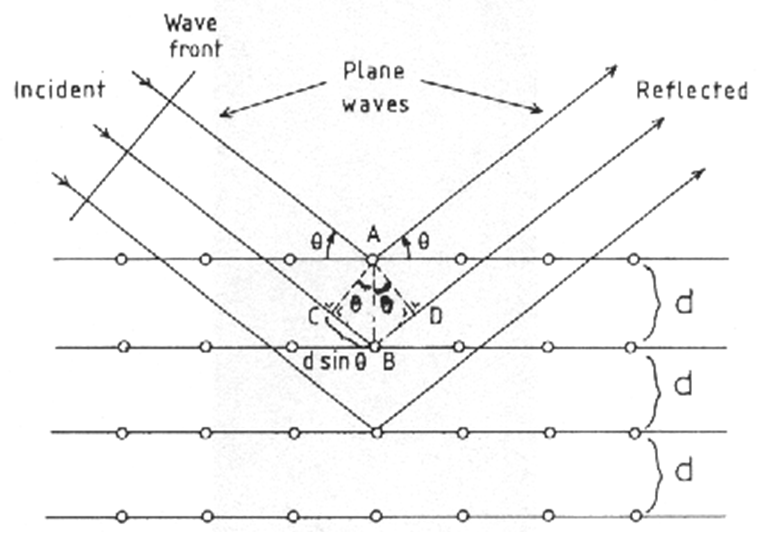
\includegraphics[width=4.0in]{./figures/Topic9/Fig9-5.png}
	\caption{ Reflection of x-rays from layers, or planes, in a crystal.}
 	\label{Fig9-5}
\end{figure}
Each atomic layer reflects a portion of the incident radiation.  From the diagram, we can see that x-ray waves that penetrate deeper into the crystal must travel farther by a distance we will label $\Delta\ell/2$; the additional path length depends on both the separation distance $d$ between layers and the angle of incidence $\theta$.  Using simple geometry, we calculate the additional path length per layer to be 
\begin{equation}\label{eqn9-1}
\Delta\ell = 2 d \sin\left(\theta\right)
\end{equation}
This value is the total spatial delay of the wave fronts upon exiting the crystal after they are reflected from successive layers.  Each reflected wave has the form $E=E_{\circ}\cos\left(kx\right)$, where $E_{\circ}$ is a constant; $k=\frac{2\pi}{\lambda}$ is the wavenumber; and the wavelength $\lambda$ is typically 0.5-1.5 $\text{\AA}$.  The total reflection of the beam, then, is the superposition of thousands of individual atomic layer reflections:
\begin{equation}\label{eqn9-2}
E=E_{\circ}\cos\left(k\cdot0\right)+E_{\circ}\cos\left(k\cdot\Delta\ell\right)+E_{\circ}\cos\left(2k\cdot\Delta\ell\right)+\cdots
\end{equation}
The first term corresponds to the surface layer, the second term to the second layer, and so on through the many layers in the crystal.  For most values of $\theta$, $\Delta\ell$ is such that these terms sum to nearly zero because about half are positive while the other half are negative.  Therefore, the total reflected radiation $E$ is very weak.  When the path length $\Delta\ell$ happens to equal a multiple of $\lambda$, however, the reflection is strong (constructive).  This is because the argument of each cosine term is a multiple of $2\pi$, allowing each cosine term to reach the maximum value of 1.  Thus, the condition for obtaining a strong reflection is
 \begin{equation}\label{eqn9-3}
k\Delta\ell=2\pi n, n=1, 2, 3, \cdots
\end{equation}
After substituting for$ k$ and simplifying, we get
$$\frac{2\pi}{\lambda}\Delta\ell=2\pi n$$
$$\frac{\Delta\ell}{\lambda}=n.$$
By substituting for $\Delta\ell$ from Eq.~\ref{eqn9-1} and rearranging the equation, we arrive at the famous Bragg relation:
\begin{equation}\label{eqn9-4}
n\lambda=2d\sin\left(\theta\right)
\end{equation}
If the wavelength and angle of incidence are known, then the atomic layer $d$ can be calculated with high accuracy.  

The diffraction patterns that emerge from protein crystals require much time and expertise to decipher, but the effort is rewarded by the resulting three-dimensional electron density map.  Figure \ref{Fig9-6} shows such a map for a small portion of a molecule at three different resolutions.  The detail is greatly enhanced by increasing the resolution from 3 $\text{\AA}$ to 1.2 $\text{\AA}$ -- the ring structure of a phenylalanine side chain becomes clear.
\begin{figure}[h]
	\centering
	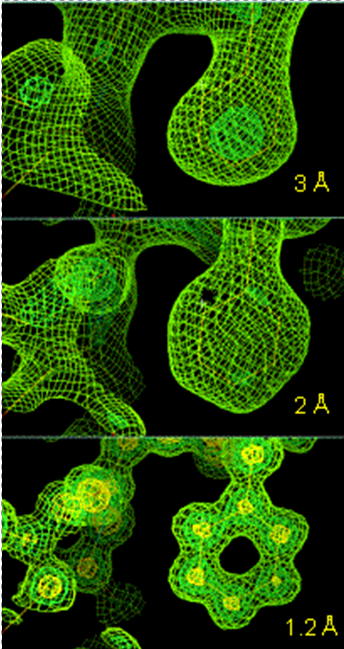
\includegraphics[width=2.0in]{./figures/Topic9/Fig9-6.png}
	\caption{ An electron density map at three different resolutions.\href{ http://www-structure.llnl.gov/Xray/101index.html}{ http://www-structure.llnl.gov/Xray/101index.html}}
 	\label{Fig9-6}
\end{figure}
Finally, sophisticated computer graphics programs put together the data from electron density maps to produce valuable 3D images, like the one of myoglobin in Fig.~\ref{Fig9-7}:
\begin{figure}[h]
	\centering
	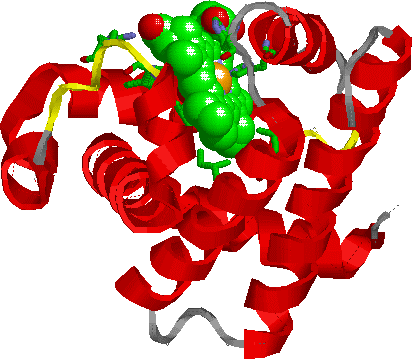
\includegraphics[width=3.0in]{./figures/Topic9/Fig9-7.png}
	\caption{ Ribbon structure of myoglobin.}
 	\label{Fig9-7}
\end{figure}

\section{Nuclear Magnetic Resonance (NMR) Spectroscopy}

Nuclear Magnetic Resonance (NMR) is the quantum mechanical phenomenon upon which two important technologies are based: NMR spectroscopy and Magnetic Resonance Imaging (MRI).  NMR spectroscopy, as we have already noted, provides information about protein structure.  Further, it aids the study of molecular dynamics, or how molecules or complexes of molecules behave in solution.  MRI uses essentially the same physical principles but for medical imaging purposes.  How NMR spectroscopy works is the focus of this section.  MRI will be discussed in Topic 10.

\subsection{The basic concept}

As the concepts behind NMR spectroscopy are highly mathematical and often unintuitive, providing an introductory-level explanation of NMR theory can be problematic.  For this reason we will begin with a classical analogue— compasses in a magnetic field — to get a sense of how NMR works, before introducing some of the quantum effects that make this type of spectroscopy so useful.

Consider a compass used for navigation, consisting of an magnet mounted on a pivot such that it can spin freely.  No matter which way the compass is turned, the magnet always settles facing geographic North.  This alignment occurs because the compass ``feels'' the pull of Earth’s own magnetic field, shown in Figure \ref{Fig9-8}.  
\begin{figure}[h]
	\centering
	
\includegraphics[width=2.0in]{./figures/Topic9/Fig9-8.jpg}
	\caption{The Earth is a giant magnet.}
 	\label{Fig9-8}
\end{figure}
If we place the compass between the poles of a strong magnet, it will become aligned with this new magnetic field instead of with Earth's.
\begin{figure}[h]
	\centering
	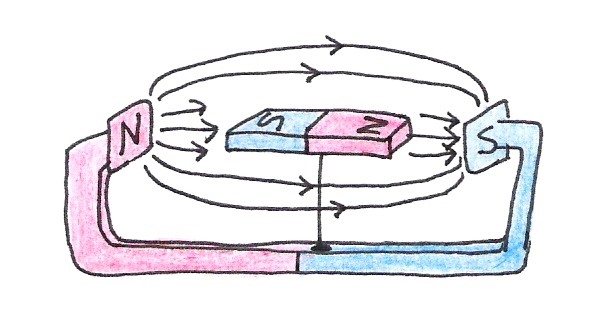
\includegraphics[width=3.0in]{./figures/Topic9/Fig9-9.jpg}
	\caption{A compass magnet aligns itself with an external magnetic field.}
 	\label{Fig9-9}
\end{figure}
Once the compass is aligned, it will remain in the same position until the external field changes or the magnet itself is disturbed.  Imagine rotating the magnet gently with your finger so that it is out of alignment with the external field (See Fig.~\ref{Fig9-10}).
\begin{figure}[h]
	\centering
	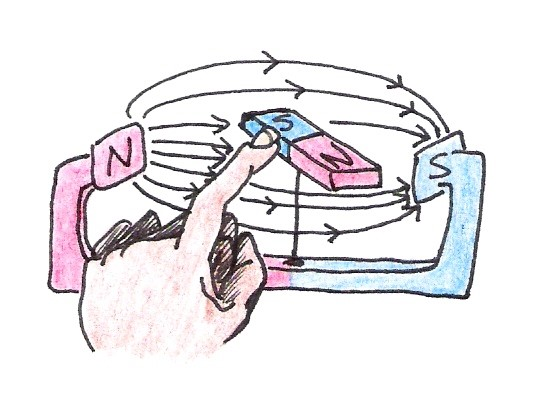
\includegraphics[width=3.0in]{./figures/Topic9/Fig9-10.jpg}
	\caption{ An external disturbance causes the magnet to become misaligned with the external magnetic field.}
 	\label{Fig9-10}
\end{figure} 
When you let it go, the magnet swings back towards equilibrium but continues past it due to momentum.  Then it swings back in the other direction.  The magnet continues to oscillate in this way until the frictional forces at the pivot bring the magnet to rest, again aligned perfectly with the field.  Figure \ref{Fig9-11} shows the angle of the compass needle measured with respect to the equilibrium position as a function of time.
\begin{figure}[h]
	\centering
	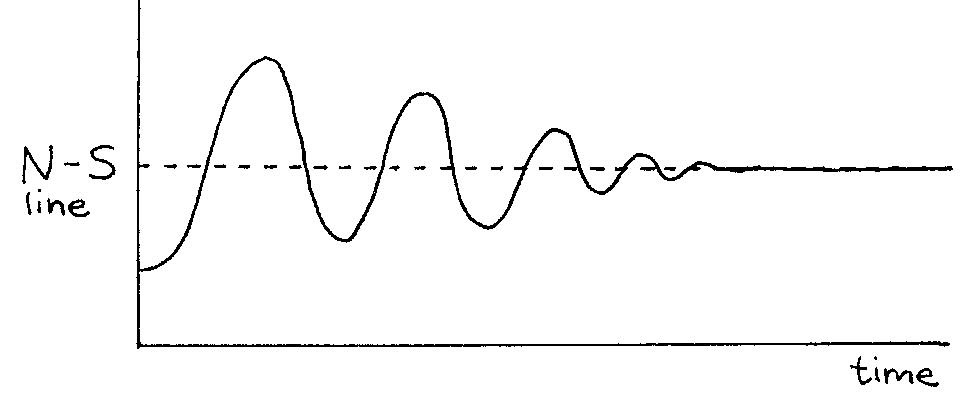
\includegraphics[width=4.0in]{./figures/Topic9/Fig9-11.jpg}
	\caption{Motion of a perturbed compass magnet in an external magnetic field.}
 	\label{Fig9-11}
\end{figure} 
Two factors affect the frequency of the oscillatory motion: the strength of the external magnetic field and the ``strength'' of the compass magnet itself.  If the compass is placed in a stronger magnetic field, or if the compass magnet itself is stronger, the frequency increases.  In other words,
$${\rm Frequency}\propto{\rm external~field~strength}\cdot{\rm compass~field~strength}$$
We can determine the strength of the compass magnet by knowing the magnetic field strength and by measuring the frequency of oscillation.  Let us now look at how we measure this frequency.

According to Faraday's law of induction, a magnetic field that changes its strength induces a voltage in a nearby loop of wire.  If we place a wire loop near our compass and perturb it as before, the loop will ``feel'' the changing magnetic field emanating from the moving compass.  The resulting voltage will oscillate with the same pattern as the magnetic field shown in Figure \ref{Fig9-12}. We can directly measure this electric effect directly with instruments such an oscilloscope.  This means that we can electrically characterize the oscillatory motion of compass' field.  
\begin{figure}[h]
	\centering
	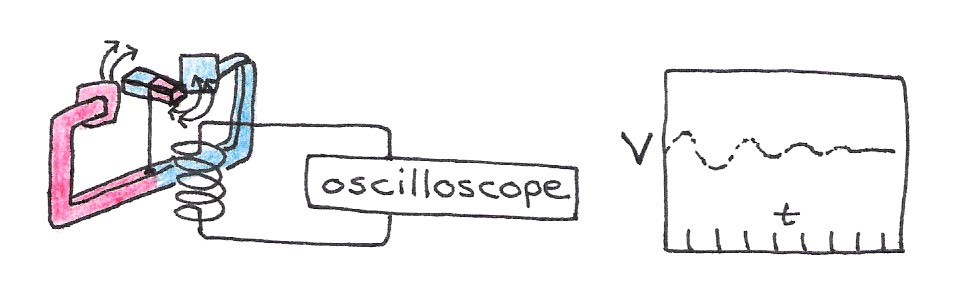
\includegraphics[width=5.0in]{./figures/Topic9/Fig9-12.jpg}
	\caption{A changing magnetic field produces a measurable voltage in a nearby wire loop.}
 	\label{Fig9-12}
\end{figure} 
What does this have to do with NMR spectroscopy?  Well, like a compass, a nucleon (a proton or neutron) acts as a magnet.  The nucleon's magnetic `` strength'' is described by a quantity called the magnetic dipole moment, denoted $\mu$.
\begin{figure}[h]
	\centering
	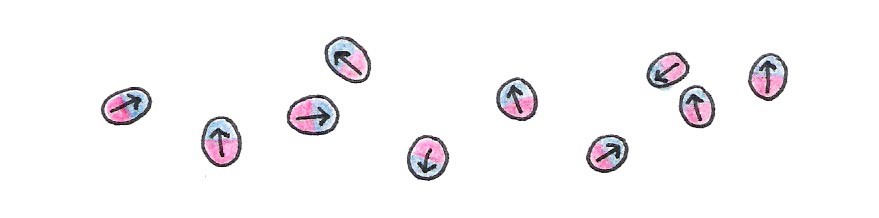
\includegraphics[width=5.0in]{./figures/Topic9/Fig9-13.jpg}
	\caption{Every nucleon possesses intrinsic magnetism.}
 	\label{Fig9-13}
\end{figure} 
Since the nucleon acts as a tiny magnet, it too has a north and a south pole.  Within a nucleus with an even number of nucleons, the north pole of one nucleon pairs up with the south pole of another so that the combined magnetic moment of the nucleus is nearly zero.  If the nucleus instead contains an odd number of nucleons, it has a net dipole moment -- a necessary condition for NMR spectroscopy.  This condition is met by the hydrogen nucleus ($^1$H), which is abundant in water and biomolecules like proteins.  Certain isotopes like $^{13}$C and $^{15}$N are also frequently used for NMR because they have a net dipole moment.

Imagine that we have prepared a sample of purified protein in solution.  The solvent is the so-called ``heavy'' water D$_2$O, made by replacing the $^1$H atoms of normal H$_2$O with $^2$H, a hydrogen isotope called deuterium.  Since $^2$H contains both a proton and a neutron, it has no net magnetic dipole moment and therefore produces no NMR signal.  Only the hydrogen atoms in the protein are then detectable.

In the absence of an external magnetic field, all the nuclear dipoles in the protein point in random directions.  When we place the sample in an external field, however, as we did with the compass in Figure \ref{Fig9-9}, we find that many of the dipoles become aligned with the field.  Assuming we could perturb the dipoles slightly, each would produce a characteristic oscillatory signal much like the one in Figure \ref{Fig9-11}.  We could then detect the signal with a wire loop and measure the frequency emitted from each dipole.

Since we cannot use our finger to create the necessary disturbance, like we did with the compass, we must find another way to disturb their alignment.  This can be  accomplished by switching on an additional magnetic field that ``pushes'' the dipoles out of alignment with the external field, causing them to oscillate  A good way to produce this additional magnetic field is to run current through a wire coil, placed orthogonal to the original external magnetic field in which our sample is placed.  
\begin{figure}[h]
	\centering
	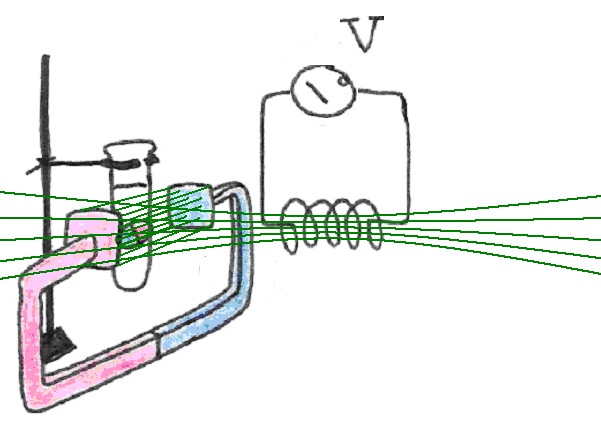
\includegraphics[width=3.0in]{./figures/Topic9/Fig9-14.png}
	\caption{The addition of a sudden, transverse magnetic field,  displaces the magnetic dipoles from their equilibrium orientation relative to the main field.}
 	\label{Fig9-14}
\end{figure} 

In order to elicit sizable signals from samples it is important to generate significant re-orientation of the magnetic dipoles within. One way to create those large angular displacements of the magnetic dipoles is to switch on suddenly a very strong magnetic field. Unfortunately, the field strength required would be so strong to make it impractical. Instead a technique based on the concept of resonance is used. Here, a field is produced that changes polarity periodically, thus forcing the magnetic dipoles to twist back and forth. When the frequency of the field is synchronized with the oscillatory motion of the dipoles within the big magnet, resonance takes place. This phenomenon is akin to a child ``pumping'' a swing into motion by rotating the entire body at the points of highest displacement. Every time the child performs this maneuver a bit of energy is added to the motion which thus continues to grow. A diagram is shown in Fig.~\ref{Fig9-15}. 
 \begin{figure}[h]
	\centering
	\includegraphics[width=4.0in]{./figures/Topic9/Fig9-15.png}
	\caption{A child on a swing pumps the swing's motion.}
 	\label{Fig9-15}
\end{figure} 

\subsection{Angular Momentum Effects}

Due to angular momentum effects, the oscillatory signal from the dipole does not arise in quite the same way as it does from the compass.  In quantum mechanics, there is a direct connection between the magnetic dipole moment of a particle and its intrinsic angular momentum. In a sense, it is as if the spinning of a particle leads to the charge inside of it to move in a circle and therefore to act as a small electromagnet. Thus, each nucleon with a magnetic dipole moment also possesses angular momentum with a axis of rotation aligned with the south-north pole..     
As a rule, whenever a body spinning about an axis is subjected to a torque (a turning force), its axis of rotation precesses.  Picture a bicycle wheel with one end of its axle tied to a string as shown in Fig.~\ref{Fig9-16}.  If we hold the wheel upright and let it go, the force of gravity causes it to fall and oscillate like a pendulum, just as we would expect. This kind of motion is similar to that of the compass in a magnetic field.
\begin{figure}[h]
	\centering
	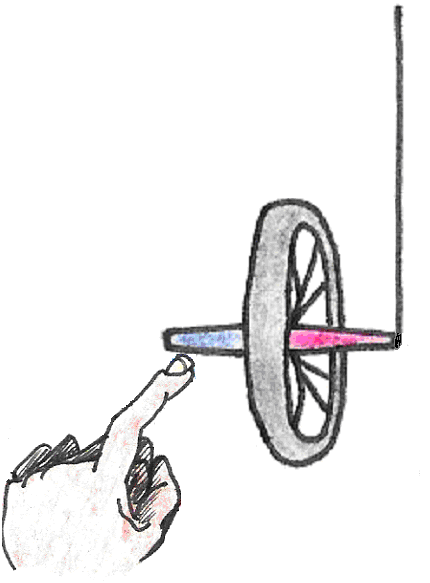
\includegraphics[width=2.0in]{./figures/Topic9/Fig9-16a.png}
           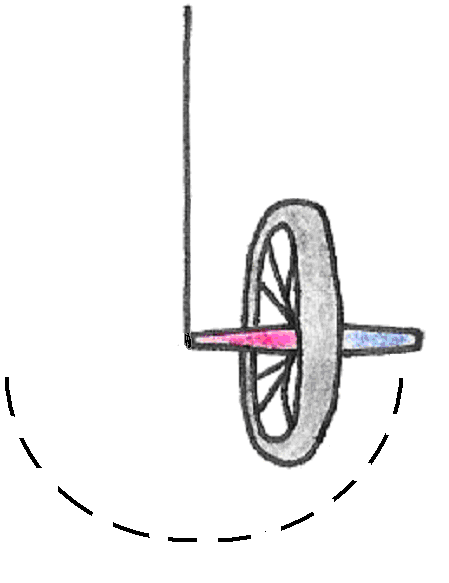
\includegraphics[width=2.0in]{./figures/Topic9/Fig9-16b.png}
	\caption{Motion of a static bicycle wheel.}
 	\label{Fig9-16}
\end{figure}
If, on the other hand, we hold the wheel upright and begin to spin it before letting go, the wheel will remain upright but will also turn about the axle, or precess (Fig.~\ref{Fig9-17}).  
\begin{figure}[h]
	\centering
	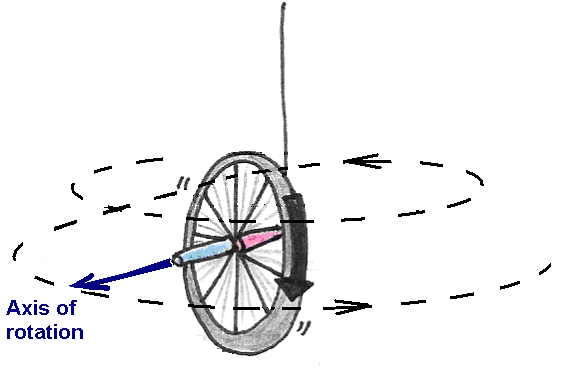
\includegraphics[width=3.0in]{./figures/Topic9/Fig9-17.png}
	\caption{Precession of a spinning bicycle wheel.}
 	\label{Fig9-17}
\end{figure} 

To see why the bicycle wheel undergoes this circular motion, let us look at the forces acting upon it. These are shown in Figure \ref{Fig9-18}.
\begin{figure}[h]
	\centering
	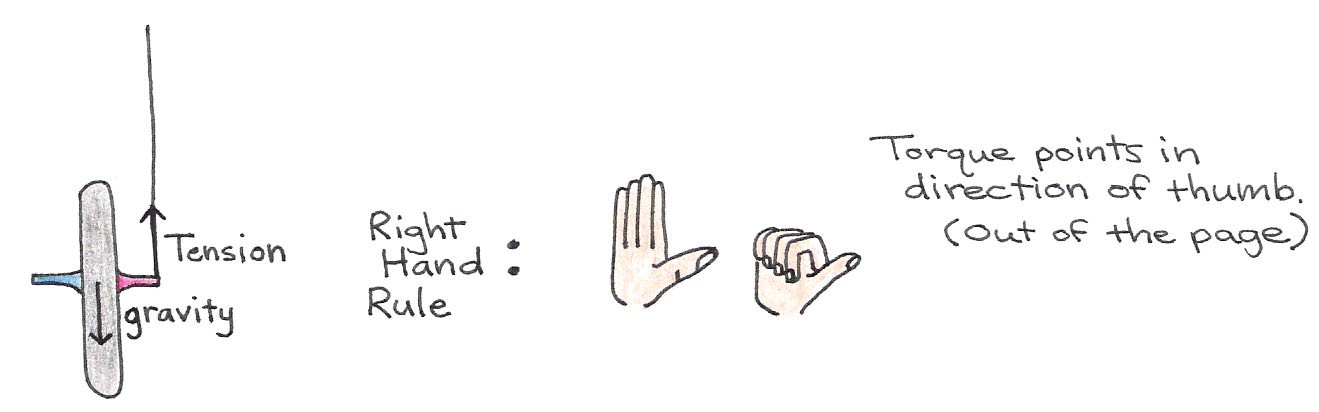
\includegraphics[width=\textwidth]{./figures/Topic9/Fig9-18.jpg}
	\caption{Forces acting on the bicycle wheel, which produces a torque.}
 	\label{Fig9-18}
\end{figure} 
On one end of the axle, the string exerts a tension force normal to the wheel’s axis of rotation.  The force due to gravity acts in the opposite direction of this tension force, but it is applied at the center of mass—the middle of the wheel.  Because the forces are not collinear, there is a torque applied on the wheel that exerts a counter-clockwise turning force. In the absence of spinning, the torque causes the bicycle wheel to swing down freely in the manner shown in Fig.~\ref{Fig9-16}. However, if the wheel is spinning to begin with, i.e., if it has an angular momentum to begin with, it can no longer swing down freely as before. To understand why, refer to Fig.~\ref{Fig9-18}. In this case, the applied torque is perpendicular to the $z$-axis, which implies that the angular momentum along the $z$ remains unchanged (conserved). Therefore, a change in direction of the angular momentum of the spin must be accompanied by an opposing change elsewhere in the body, if the total angular momentum along the $z$ is to be preserved.
\begin{figure}[!htb]
	\centering
	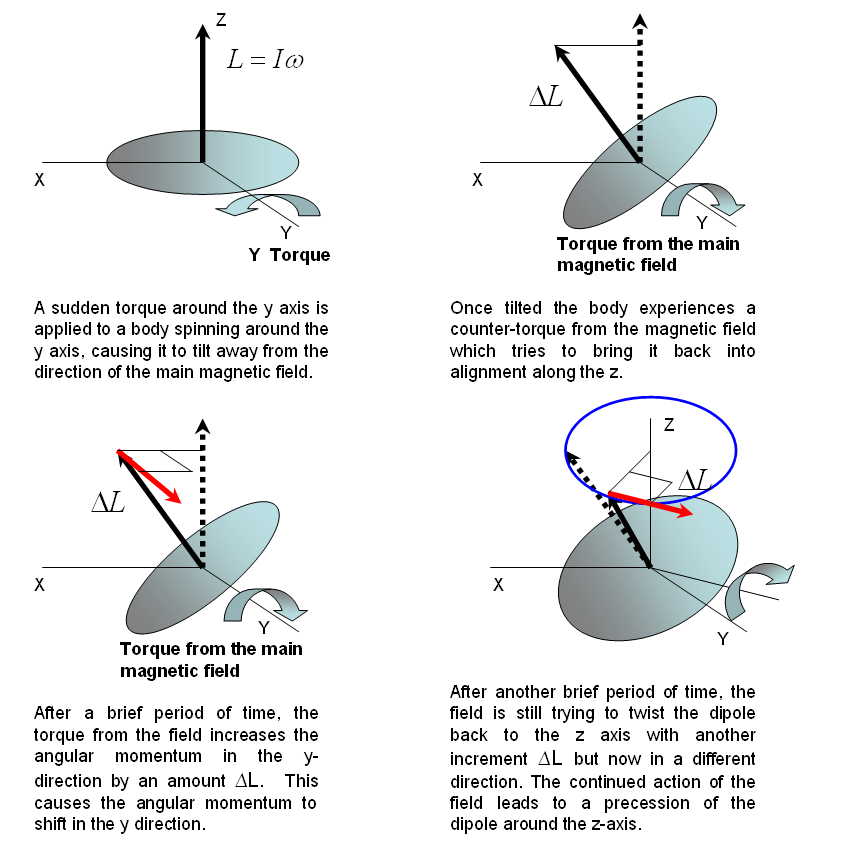
\includegraphics[width=\textwidth]{./figures/Topic9/Fig9-19.png}
	\caption{Precession caused by a torque exerted on a spinning body.}
 	\label{Fig9-19}
\end{figure} 

Let us say that the main magnetic field is applied along the $z$-direction. Before a transverse magnetic field is applied, the magnetic dipoles are lined up along the $z$-direction. When a transverse field is applied and a torque is exerted on the magnetic dipoles, they will precess in the plane perpendicular to the main magnetic field. The precession of the magnetic dipole results in a magnetic field that sweeps that transverse plane and that be picked up by an external coil as shown in Fig.~\ref{Fig9-19}. Consequently, the frequency of the signal we measure is really the frequency of precession.  In NMR spectroscopy, we call this resonant frequency the Larmor frequency.
\begin{figure}[!htb]
	\centering
	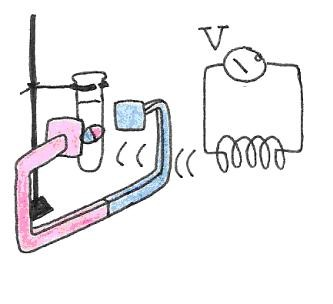
\includegraphics[width=3.0in]{./figures/Topic9/Fig9-20.jpg}
	\caption{The precession of the magnetic dipole generates a magnetic field that sweeps the plane perperdicular to the main magnetic field. The changing flux is captured by a neaby coil, resulting in an induced voltage. }
 	\label{Fig9-20}
\end{figure} 

As soon as the current in the orthogonal coil is turned off, the transverse magnetic field ceases to exist.  The dipoles slowly stop precessing, finally regaining their alignment with the external magnetic field.  The resonance spectrum produced for a single dipole -- or a sample in which only one type of dipole exists, like H$_2$O -- looks very much like that of the compass in Figure \ref{Fig9-11}. This frequency is the Larmor frequency.

As we argued earlier, the frequency of oscillation of a compass depends on both the strength of the external magnetic field and the strength of the compass magnet itself.  In the same way, the Larmor frequency of a nuclear magnetic dipole increases with external field strength and varies according to the identity of the dipole.  For instance, $^1$H nuclei have a characteristic frequency that is different from that of $^{15}$N nuclei.  To see which types of dipoles are present in a sample, we use a process called a Fourier Transformation.  This technique mathematically characterizes the frequencies of the waves present in the raw NMR data (e.g. Figure \ref{Fig9-11}) in terms of their frequencies.  If we look at a single dipole, as suggested in Fig.~\ref{Fig9-19}, there will be only one wave and thus one frequency. The NMR spectrum will only have one peak, as shown in Fig.~\ref{Fig9-20}.
\begin{figure}[!htb]
	\centering
	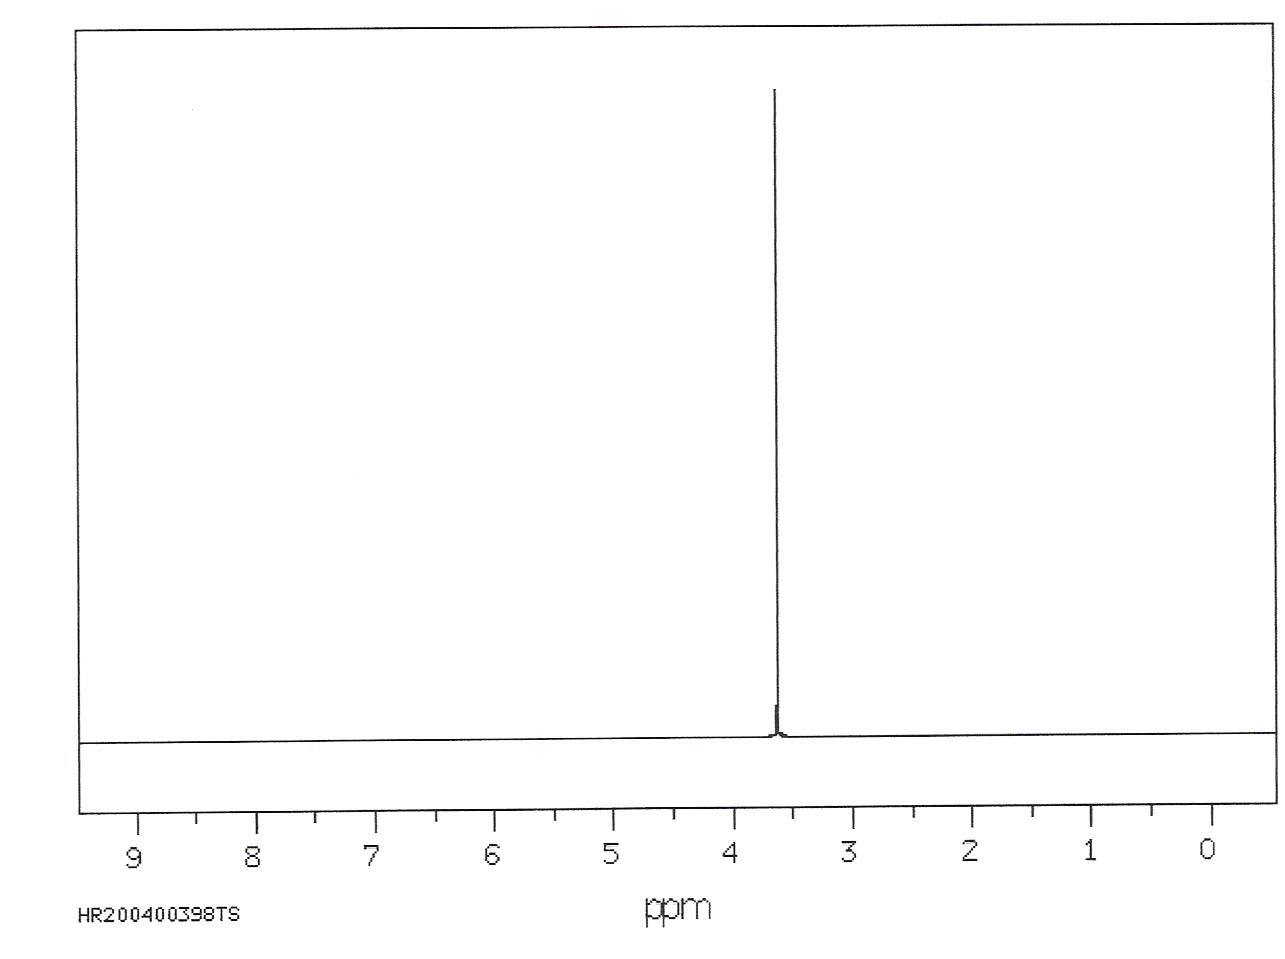
\includegraphics[width=4.0in]{./figures/Topic9/Fig9-21.jpg}
	\caption{NMR spectra show the frequencies associated with differing nucleons. In this case, the existence of a single frequency suggests that all nucleons behave identically. }
 	\label{Fig9-21}
\end{figure} 

\subsection{Chemical Shifts}

All isolated protons resonate at the same frequency, but when placed within molecules they are affected by a variety of effects such as {\it electron shielding} and {\it spin-spin coupling}. These effects cause their frequencies to shift slightly and to different extents depending on their interaction with electrons and other nucleons within the molecule. These shifts are known as chemical shifts. These shifts are small -- on the order of parts per million (ppm) -- but it is detectable by NMR spectroscopy. By analyzing the shifts of an NMR spectrum, we can derive the structure of the molecule.

In {\it electron shielding}, the shift arises from the interaction of the electrons and the nuclear magnetic field. To understand these effects, we return to the compass analogy.  Imagine that we place our compass close to a material that can become magnetized. The magnetic field from the compass can magnetize the material, turning it into another magnet. This newly induced magnet can in turn affect the overall magnetic field that the compass is subjected to. Now consider the hydrogen atom, consisting of a proton with an electron revolving around it, placed inside a magnetic field.  Like the material near the compass, the electron orbit is altered (magnetized) slightly due to its close proximity to the proton’s magnetic field, and now begins to emanate its own magnetic field. This field partially negates the one produced by the main field, leading to a small reduction in the overall magnetic field the nucleon is subjected to. This results in a small reduction or shift of the Larmor frequency produced by the nucleon.

{\it Spin-spin coupling} involves interactions of a nuclear magnetic dipole with neighboring ones. When magnetic dipoles are close together, typically within three bond lengths, the magnetic field of one affects the overall magnetic field the other experiences. Nuclear spins like electron spin, is quantized such that it can only assume one of two orientations in a magnetic field: up or down. As a result, the Larmor frequency of a proton increases or decreases slightly depending on the orientation of this nearby spin, i.e. whether the latter are up or down.  The NMR spectrum of either nuclei is split into two peaks in this case, as shown in Fig.\ref{Fig9-22}. By quantifying the small differences in their frequencies, we can infer also their proximity. If more than two nuclei are in close proximity, the spectrum exhibit splitting patterns that are increasingly complex, but still can be worked out.
\begin{figure}[!htb]
	\centering
	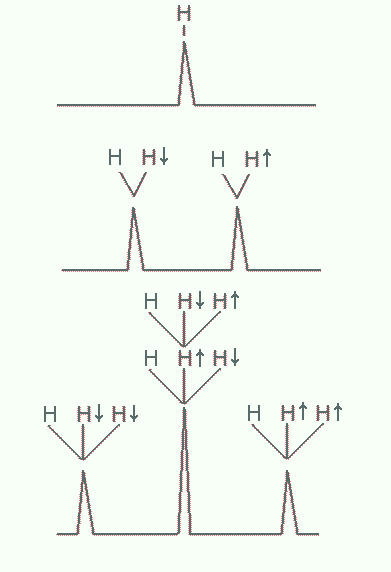
\includegraphics[width=2.5in]{./figures/Topic9/Fig9-22.png}
	\caption{ Splitting of NMR resonances due to spin-spin coupling}
 	\label{Fig9-22}
\end{figure}

Take note that in the examples above we worked out the spectrum from knowledge of the molecular structure.  The usual practice in NMR spectroscopy is to obtain a spectrum and then use it to solve the structure of the molecule.  The process for determining the structure of a protein is essentially the same as for a simple molecule, except that the spectrum is decidedly more complex due to the large number of hydrogen atoms present.  Figure \ref{Fig9-23} shows an NMR spectrum for a small protein.
\begin{figure}[!htb]
	\centering
	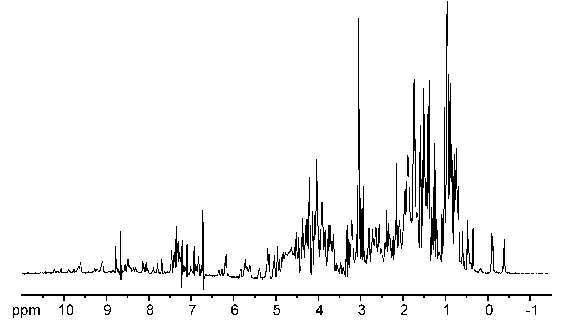
\includegraphics[width=4.0in]{./figures/Topic9/Fig9-23.png}
	\caption{NMR spectrum of a small protein.}
 	\label{Fig9-23}
\end{figure} 

\subsection{Beyond Simple Spectra}

Several ingenious techniques help us overcome the difficulty of analyzing such complex spectra.  For instance, you can make a set of nuclear spins to precess and probe how those affect the precession of others. You can also incorporate NMR-active isotopes, like $^{15}$N, into the protein.  To do this, protein samples are derived from cells grown in a special medium containing $^{15}$N.  This ensures that when the cells begin expressing the protein of interest, the amino acids will be labeled with the heavier isotope needed for resonance.  You can then run a spectroscopic experiment that correlates directly-bonded $^{1}$H and $^{15}$N atoms.  These techniques give rise to two-dimensional spectra, containing additional information that helps one determine the protein structure.

One additional challenge must be considered to structurally characterize a protein, since NMR spectroscopy is performed on proteins in solution, we must incorporate theory of molecular motion into our analysis.  Since many proteins have regions that flop around -- particularly the ends --we almost always end up with several dozen “probable” structures.  The average of these is taken to be the structure of the protein under the experimental conditions.

The fact that we cannot determine a definitive structure for the protein using NMR spectroscopy may at first seem like a disadvantage, but it is in large part why the method is so useful: unlike x-ray crystallography, NMR gives us a more realistic approximation of how proteins behave {\it in vivo}. 
